\documentclass{article}[12pt]
\usepackage[utf8]{inputenc}
\usepackage{graphicx}
\usepackage[a4paper,width=150mm,top=25mm,bottom=25mm,bindingoffset=6mm]{geometry}
\usepackage{amsmath,amssymb}
\usepackage{subfig}
\usepackage{setspace}

\usepackage{caption}

\usepackage{ntheorem} % For writing hypotheses
\theoremseparator{:} % Insert :

\newtheorem*{hyp*}{Hypothesis \protect\hypnumber} % Name "Hypothesis"
\newenvironment{hyp}[1]{\renewcommand{\hypnumber}{#1}\begin{hyp*}}{\end{hyp*}}
\newcommand{\hypnumber}{}

\usepackage{xcolor}
\usepackage{xparse}
\NewDocumentCommand{\codeword}{v}{%
\texttt{\textcolor{blue}{#1}}%
}

\usepackage{cleveref}

\title{ Random Walk Modeling of Equity Indexes across Different Industries : ANOVA Comparison}
\author{ Orhan Koc \\ orhankoc@uw.edu \and
         Jyunghyun Noh \\ jyungn@uw.edu \and
         Siew Kit Liew \\ siewkit@uw.edu
    }

\doublespacing

\begin{document} 

    \begin{figure}
        \centering
        
\includegraphics[width=0.30\textwidth]{../assets/uw.png}
    \end{figure}
    \maketitle

    \begin{abstract}
        This study aims to assess how well Random Walk, or an Auto Regressive(AR) Integrated Moving Average(MA) with no AR or MA compoenents, ARIMA(0,1,0) models stock prices of different industries. Monthly price data is collected from stocks of different industries, stationarized and fit with a random walk model. The RMSE values for each model vs price data is fed into an Analysis of Variance (ANOVA) model to see if each market is as random as the other. The assessment is conducted using One-Way ANOVA to assess if there is significant difference in random walk modeling error among stocks of different industries. We will be employing Single Factor Anova design with multiple levels as different stocks, and multiple observations as randomized intervals chosen from a 5 year data fetched from FRED. 
        The results of the study will provide insights into the robustness and generalization of Random Walk ARIMA(0,1,0) model in stock price modeling in different industries. This research aims to find whether some markets are more random than the others. The findings of this study will be valuable for investors, financial analysts, and academics interested in stock price forecasting and time series modeling.
    \end{abstract}

    \newpage

    \section{Introduction}
        Since the dawn of finance, academia and the finance industry have made numerous attempts at systematically predicting the returns on risk bearing assets. The long lasting debate of whether stock markets are predictable or not has been steered towards the former with the emergence of new models. In this paper, we wish to compare the randomness of markets of different industries to ultimately understand whether some markets are more predictable than the others.

        Price forecasting is a widely studied subject usually implemented with a variety of well-tested machine learning algorithms. One of the most comprehensive ways of describing a model with forecasting capabilities is the Autoregressive integrated Moving Average, also known as ARIMA, model. The robustness of this algorithm mainly stems from the fact that it's a combination of multiple methods of modeling. One of the apparent advantages of ARIMA is it's ability to model future values solely based on past values. We will consider the simplest version of ARIMA, the random walk (0,1,0) which itself is a cumulative sum of an independent and identically distributed process, ARIMA(0,0,0). The 1 represents we will be taking the difference of the data to convert the trending prices into stationary data.        Essentially, we want to see if some markets are more random than the other. Using one-way ANOVA, we will see if there is significant difference between the RMSE of different equity indexes modeled by random walk. The equity indexes are chosen such that there is little overlap between and so that they represent different industries. The results of this experiment can be useful in determining which markets resemble a random walk less than the others with respect to different industries. 

        The data will be collected from Federal Reserve Economic Data (FRED). In order to observe difference of randomness with respect to different industries, we chose to include equity indexes of different areas of employment: Technology, Transportation, Utility etc. We include the monthly average price for SP500, NASDAQ, DOSJUA, DOWJT indexes from 2013 to 2022. We will then pick random intervals of 5 years for each observation and compare a Random Walk model to the corresponding index and record the RMSE. If all markets are equally random, than there should be no significant difference in the RMSE values for indexes, H0 is correct.
        
        \section{Theory}
        \subsection{Random Walk}
        Time series analysis of stocks to predict future prices has been a focus of research since the birth of finance. Among models that use past data alone to forecast future prices, ARIMA has been the most successful alternative. Auto-Regressive Integrated Moving Average (ARIMA) is composed of two parts:

        Autoregressive Regression (AR) is a special case of linear regression where the output $X_t$ is determined by a linear combination of past values.
        \begin{equation}
            X_t = a_1 x_{t-1} +a_2 x_{t-2} + \dots +a_p x_{t-p} +w_t 
        \end{equation}
        Moving Average (MA) attempts to state the mean for a period of time using a linear combination of past white noise. 
        \begin{equation}
            X_t = \mu + \epsilon_t + \theta_1 \epsilon_{t-1} + \dots + \theta_q \epsilon_{t-q}
        \end{equation}
        Combining signal prediction of AR and noise prediction of MA together yields the relationship stated in Eq 3, and usually outperforms both AR and MA in terms of forecast accuracy. 
        \begin{equation}
            X_t = a_1 x_{t-1} +a_2 x_{t-2} + \dots +a_p x_{t-p}w_t +  \theta_1 \epsilon_{t-1} + \dots + \theta_q \epsilon_{t-q}
        \end{equation}

		ARIMA function uses 3 parameters p,d and q: p as the lag order, d as the degree of differencing needed for stationarity and q as the order of the moving average.
	    It is important to note that our model has $p=0$ for AR component coefficient and $q=0$ for MA component coefficient, while having a differencing order of $1$. This means that we will be differencing the data once to make it stationary and compare it with white noise. When a time series data is stationary, it means the data has no significant change in mean or variance. Here is an example of NASDAQ for the first observation:

          \begin{figure}[htbp]
            \centering
            \subfloat[Nasdaq]{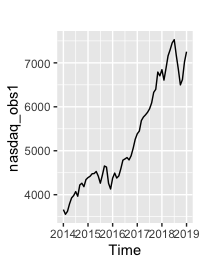
\includegraphics[width=0.4\textwidth]{../assets/nasdaq.png}\label{fig:f1}}
            \hfill
            \subfloat[Differenced Nasdaq]{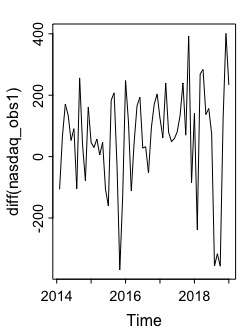
\includegraphics[width=0.4\textwidth]{../assets/nasdaq_diff.png}\label{fig:f2}}
            \caption{Original v. Stationarized}
          \end{figure}


        We will be using this Random Walk model to compare against stationarized equity index prices and record the Root Mean Squared Value for each time window. In order to make a comparison, we will be considering the difference of Random Walk or ARIMA(0,1,0) movements, also known as White Noise or ARIMA(0,0,0). The calculation of error margin for the $j$th equity index at $k$th time window is as follows:
          
        \[ y_{j,k} = \sqrt[2]{\frac{\sum_{i=1}^{N}} (\hat{y_i} - y_i)^{2}}{N} \]
          
        which is essentially the Root Mean Squared Error (RMSE) value for the White Noise model applied on stationarized data of stock $j$ during time window $k$. For an example, the $y_i$ value refers to the differentiated price seen in Figure 2 plot A, and $\hat{y_i}$ values refer to the data points in the White Noise, in Figure 2 plot B.
        
        \begin{figure}[htbp]
            \centering
            \subfloat[]{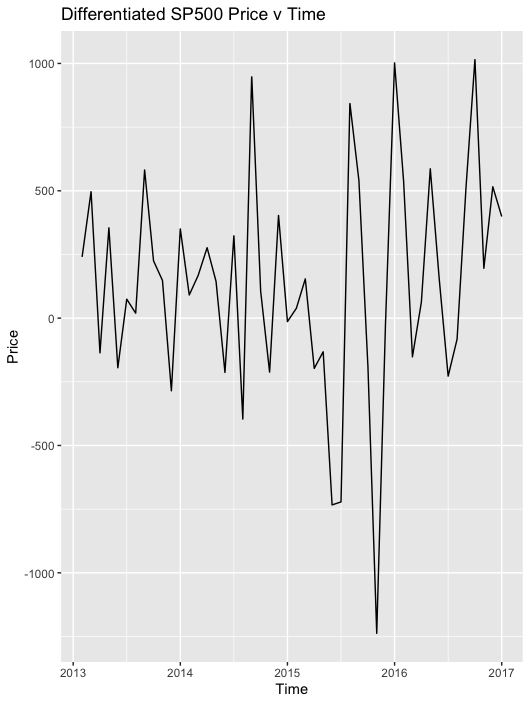
\includegraphics[width=0.48\textwidth]{../assets/diff_sp500.png}\label{fig:f1}}
            \hfill
            \subfloat[]{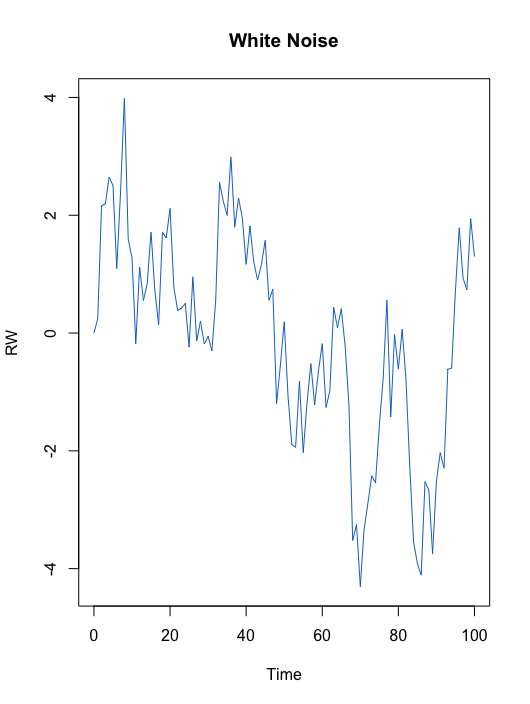
\includegraphics[width=0.52\textwidth]{../assets/whitenoise.png}\label{fig:f2}}
            \caption{Differentiated Data v. White Noise}
          \end{figure}

          Its important to realize the magnitude of the steps as well as the starting point $x_0$ in White Noise model will be adjusted with respect to $k$th time range of $j$th asset during comparison and RMSE calculation.

        \subsection{One Way ANOVA}
        Analysis of Variance (ANOVA) is a statistical technique that is used to determine whether there is a significant difference between the means of two or more groups. The ANOVA test is used when there are multiple groups, and we want to compare the means of each group to determine whether there is a significant difference between them. The ANOVA test is based on the assumption that the data is normally distributed and that the variances of the different groups are equal.

        The basic idea behind ANOVA is to compare the variation between groups to the variation within groups. If the variation between groups is much greater than the variation within groups, then there is a significant difference between the groups, and we can reject the null hypothesis. The null hypothesis for ANOVA is that there is no significant difference between the means of the groups, and the alternative hypothesis is that there is a significant difference between the means of the groups. The test is based on the F-statistic, which is the ratio of the variation between groups to the variation within groups. If the F-statistic is large, then there is a significant difference between the means of the groups, and we can reject the null hypothesis.
        
        There are different types of ANOVA tests depending on the number of groups being compared and the type of experimental design. We will be using a One-way ANOVA when there is only one independent variable, and it has more than two levels. The single independent variable is Equity indexes and the levels are different combination of stocks forming different equities
        
    \section{Experiment Design}

    \textbf{Sampling Unit} 
    This study sample consisted of three different stocks as multiple levels of a single factor ANOVA design. These stocks are all featured by the huge market cap between $10 billion and $200 billion and their shares mostly belong to public hands. In the other word, the stock prices are less likely to be manipulated by other nonsignificant factors and the asset is less volatile since the market is well established and therefore the data is more reliable. In order to address the infinitesimal issue with ARIMA model and increase the accuracy of experimental outcomes, the input data was converted into monthly price and set as the range of our data.
    
    \textbf{Equipment}
    As the intention of our study is to test the validity of ARIMA model, we utilized the 5 years of dependable data for input from Kaggle. Since we are dealing with time series data and model adequacy, we used \codeword{tseries} to work with tseriesd data and generate Random Walk and \codeword{ggplot} is used to visualize data. The experiment will use Analysis of Variance with a Randomized Complete Block Design, where observations (time intervals) will be used as blocks, where time intervals will be of same length, chosen at random for block.

    \medskip
          \begin{center}
            \begin{tabular}{ |p{2cm}||p{2cm}|p{2cm}|p{2cm}|p{2cm}|}
                \hline
                \multicolumn{5}{|c|}{Stock | Observations} \\
                \hline
                Equity Index&$t_{1}$      &$t_{2}$    &$t_{3}$    &$t_{4}$    \\
                \hline
                NASDAQ      &$y_{1,1}$   &$y_{1,2}$  &$y_{1,3}$  &$y_{1,4}$  \\
                SP500       &$y_{2,1}$   &$y_{2,2}$  &$y_{2,3}$  &$y_{2,4}$  \\
                DOWJU       &$y_{3,1}$   &$y_{3,2}$  &$y_{3,3}$  &$y_{3,4}$  \\
                DOWJT       &$y_{3,1}$   &$y_{3,2}$  &$y_{3,3}$  &$y_{4,4}$  \\
                \hline
            \end{tabular}
            \captionof{table}{Observations Table} 
    \end{center}

        \begin{hyp}{0} 
            Mean forecasting error of ARIMA(0,1,0) is statistically the same across equity idnexes of different industries, markets are equally random $\mu_{1}$ = $\mu_{2}$ = $\mu_{3}$ \dots $\mu_{n}$  
        \end{hyp}
        \begin{hyp}{1} 
            Mean forecasting error of ARIMA(0,1,0) is statistically different in at least one equity index, some markets are less random than the others $\mu_{a} \neq \mu_{b}$ where \( \mu_{a},\mu_{b} \in \{\mu_{1}, \mu_{2},\mu_{3}, \dots, \mu_{n} \} \)
        \end{hyp}

    
        \textbf{Dependent Variable} of this experiment is the error margin of the price forecasted from ARIMA(0,1,0). 
        \medskip

        \textbf{Independent Variable} of this experiment are stock prices from different industries, with multiple levels representing different stocks with the following tickers:

        \section{Data Processing}
            \subsection{Preprocessing}
                \textbf{Granularity} 10 years monthly price data fetched from Fred for S\&P500 companies and loaded into R workstation. To address known performance issues of ARIMA, daily data was converted into monthly price average data with a frequency of 12 from FRED's Graphical User Interface.

                \textbf{Stationary Data} ARIMA works best on data with no trend and constant variance. Most financial instruments, including stock prices have a trend with non-constant variance. In order to prepare the data for ARIMA timeseries forecast, we will compute the difference of logs for each data set and conduct a Dick \& Fuller's (DF) test. The  results of the function \codeword{adf.test(data)} from \codeword{library(tseries)} on the differenced timeseries data \codeword{diff(ts_obs1)}, will yield a p-value where 
                \begin{hyp}{0} 
                    $p>0.05$, Time series data is not stationary.
                \end{hyp}
                \begin{hyp}{1} 
                    $p<0.05$, Time series data is stationary
                \end{hyp}
                meaning time series with a DF result of $p<0.05$ are workable with ARIMA. For time series that failed DF test the first differentiation will be differenced again.

                \textbf{Date} Date format should be converted to MM-DD-YY in order to create a timeseries object R can work with.

            \subsection{Data Collection}
                In order to test the generalization of ARIMA, will be testing index prices of securities from different industries. We will be looking at SP500, NASDAQ, DJIA, DJTA 
                
                A quantitative difference regarding securities of different industries is the change in volatility and trend strength. This apparent difference in volatility among indexes was not chosen by the experimenters, but rather a natural result due to the change in risk appetites of the investors of corresponding industries.

        \section{Results}


        \section{Discussion}
            \subsection{Evaluation}
            [EVALUATION OF ]
                
            [EVALUATION SUMMARY]

            \subsection{Limitations \& Future Work}
                As is the case for most experiments, we expect to see more accurate results with a replication on a higher scale.

                \textbf{Observations:} Due to time constraints of course schedule, we were only able to conduct the experiment for 4 different time windows. In order to observe the appearance of Random Walk, we need to collect more observations to make sure the hypothesized independent and identically distributed behavior of markets converge.

                \textbf{Levels:} Also the number of levels of independent variable, equity indexes, were limited to four - which in return increases the room for error. If we had included more levels of our independent variable,
                
                \textbf{Overlap:} As much as we tried to pick indexes so that they have small overlap in terms of stocks included, the prominent indexes such as SP500 include a wide range of popular assets, which are also chosen by other indexes. This small but direct correlation between levels of independent variable hinders the accuracy of the experiment.

            \section{Conclusion}
                In this paper, we have conducted ANOVA on the observations of White Noise RMSE for 4 different equity indexes; repeated the observation for randomly selected time windows out of the available data for four different times. We aimed to find out if the White Noise mean RMSE for each equity index is the same across different industries. We fit White Noise models and recorded the RMSE a total of 16 times and run the ANOVA test.

                [RESULT SUMMARY]

                [EVALUATION SUMMARY]

        \section{Appendix}

    \bibliography{Biblio.bib}
    \bibliographystyle{plain}

\end{document}